\section{Постановка задачи}
\label{sec:Chapter1} \index{Chapter1}

Как уже было сказано в \autoref{sec:Chapter0}, в работе будет произведена оценка систем классификация движений человека на изображении. Из рисунка надо получить данные о принимаемой субъектом позе и классифицировать её на род деятельности. Получается решается две задачи: предобработки данных, то есть извлечение расположения ключевых точек на теле человека, и их последующая категоризация. Рассмотрим их по отдельности.


\subsection{Задача распознавания ключевых точек на теле человека}
\label{subsec:Theory of keypoint detection}

Первоначально необходимо понять каким образом можно распознать позу человека, чтобы в дальнейшем взять оттуда информацию для классификации. Человек смотрит на другого человека и анализирует его позицию исходя из данных о его расположении частей тела анализируемого. Получается нам необходимо найти части тела человека, каждая из которых ограничена какими-либо суставами. Последние можно и взять за ключевые точки, которые будут распознаваться моделью. Если соединить выходные данные, то получим своеобразный "скелет"{} человека.

Необходимо определиться сколько точек на теле человека необходимо различать. На текущий момент стандартом является топология СОСО (см. \autoref{fig:COCO_topology}), которая включает в себя 17 ориентиров на теле человека \cite{COCO_topology, COCO_dataset}. Данная топология не учитывает расположение ступней и кистей рук, а также рассматривает всего 5 точек на лице человека: нос, два глаза и два уха. Но стандартом многие исследователи не ограничиваются и добавляют дополнительные точки. Приведу два примера:

\begin{enumerate}
 \item Топология от BlazePose (см. \autoref{fig:BlazePose_topology})\\
 Включает в себя 33 точки расположенные на теле человека. Данная топология представляет собой объединение COCO, BlazeFace \cite{BlazeFace} и BlazePalm \cite{Hands}. В итоге, извлекается дополнительная информацию о направлении стоп и кистей, а также больше понимаем насчет точек на лице. Данная модель расположения точек используется в одноименной модели (BlazePose \cite{BlazePose}) и ориентирована на использование в фитнес приложениях. Также у данной компании есть более развитая модель, которая определяет положение всех пальцев кисти и распознает мимику на лице \cite{Holistic}.
 \item Halpe (см. \autoref{fig:Halpe_topology})\\
 Данная топология - это совместный проект AlphaPose \cite{fang2017rmpe} и HAKE \cite{li2020pastanet}. Представлено две модели: на 26 и на 136 точек. Здесь добавлено рассмотрение ориентации стоп, распознавание шеи, паха и макушки головы. В расширенной модели присутствует ещё 68 точек на лице, а также по 21 на ладонях.
\end{enumerate}

\begin{figure}[h]
\begin{subfigure}[b]{.3\textwidth}
	\centering
	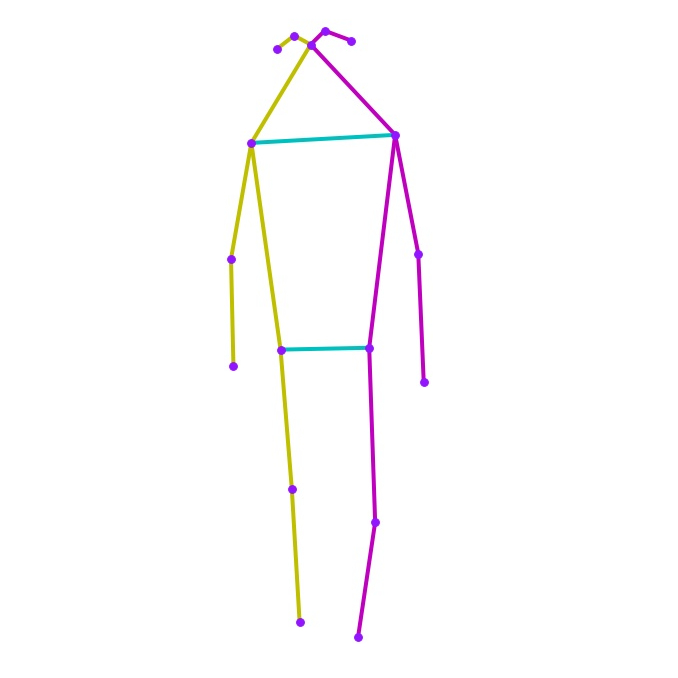
\includegraphics[width=\textwidth]{./images/COCO_topology.jpg}
	\caption{Топология COCO}
	\label{fig:COCO_topology}
\end{subfigure}
\begin{subfigure}[b]{.3\textwidth}
	\centering
   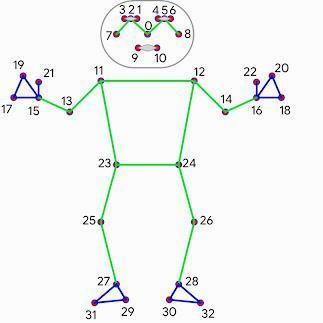
\includegraphics[width=\textwidth]{./images/BlazePose_topology.jpg}
   \caption{Топология BlazePose }
   \label{fig:BlazePose_topology}
\end{subfigure}
\begin{subfigure}[b]{.3\textwidth}
	\centering
   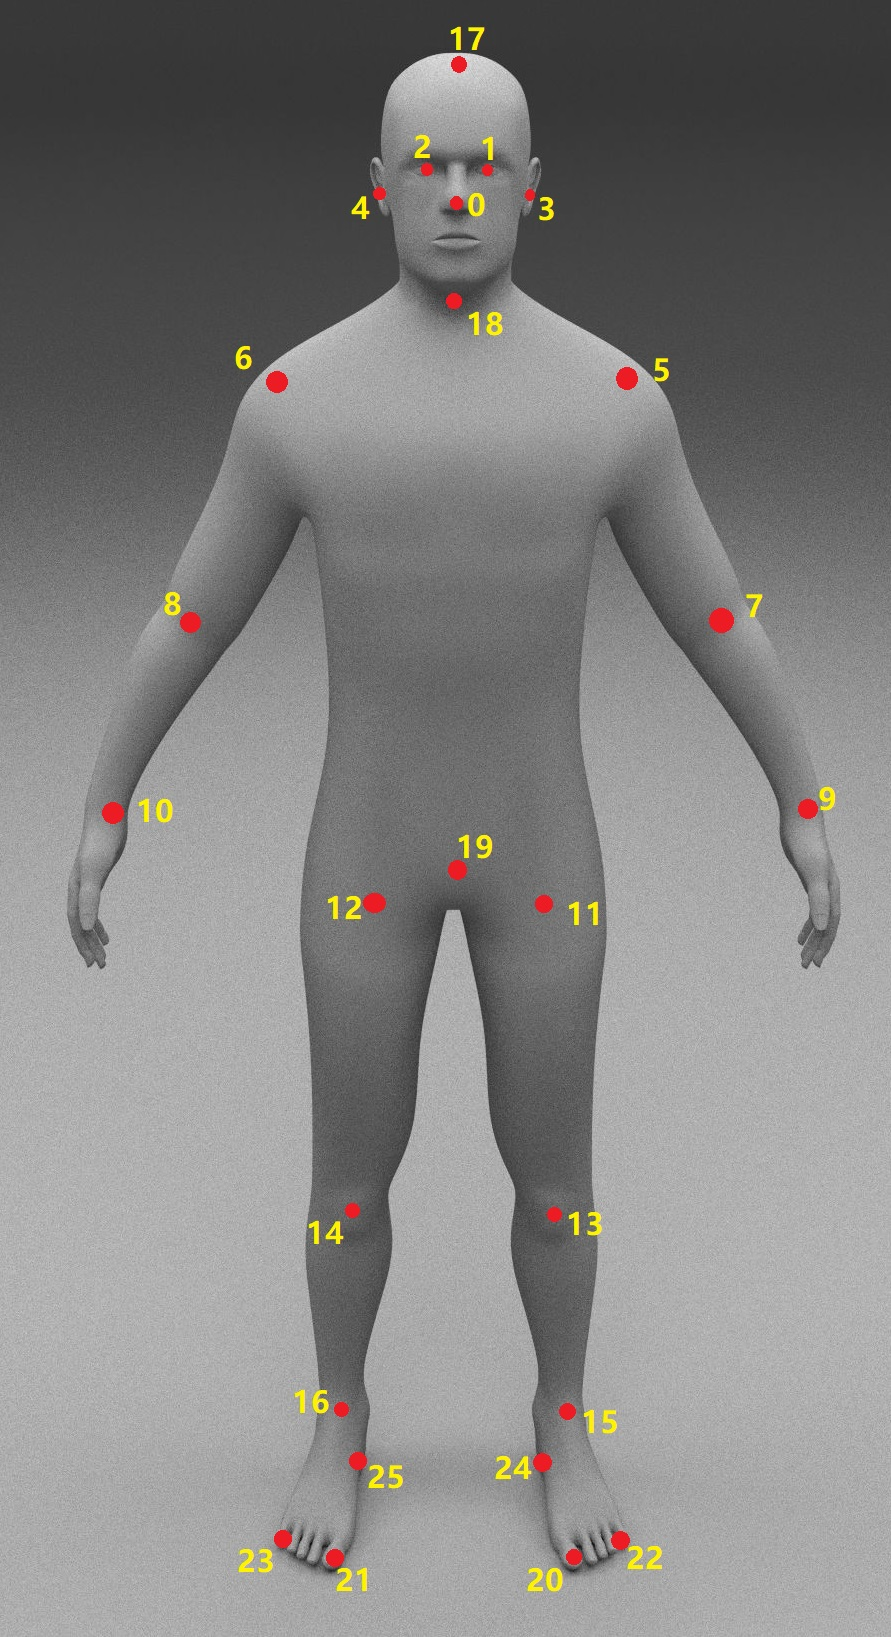
\includegraphics[height=\textwidth]{./images/Halpe_topology.jpg}
   \caption{Топология Halpe}
   \label{fig:Halpe_topology}
\end{subfigure}
   \caption{Примеры расположения точек на теле человека.}
\end{figure}

В итоге получилось разобраться с тем, что надо искать на изображении. Теперь надо выяснить каким образом искать ключевые точки на фотографии. На сегодняшний день есть два подхода:

\begin{itemize}
	\item Bottom-up\\
	Изначально строится карта предсказания для каждой ключевой точки из топологии и потом эти точки определенным образом собираются в скелет человека. Важно отметить, что при распознавании нескольких человек необходимо правильно сопоставить точки каждому человеку.
	
	Bottom-up удобно использовать при покадровой обработке видеофрагментов.
	\item Top-down\\
	В данном подходе требуется локализация человека, получение прямоугольника с ним и перенаправление этого прямоугольника в модель распознавания ключевых точек.
	Модели, использующие данный подход выдают точные результаты, но чувствительны к ошибкам детекции и к ориентации человека в кадре. Поэтому им требуется предобработка прямоугольника с человеком.
\end{itemize}

В обоих подходах результатом необходимо получить набор координат точек по заранее заданной топологии для дальнейшего преобразования в скелет человека.

\subsection{Задача классификации движений человека}
\label{subsec:Theory of classification}

Задача классификации подразумевает обучения алгоритма на размеченных данных предсказывать класс объекта исследования. К примеру можно предсказывать класс объекта на фото, тему текста, жанр музыки или позу человека.

Получается имеется множество объектов $X$, множество классов $Y$ и некоторая зависимость $cls: X \rightarrow Y$, то есть $\forall x \in X\;\exists\:y \in Y\,: y = cls(x)$. Задача классификатора состоит в том, чтобы построить алгоритм $a_cls$, который мог бы предсказывать метку из $y \in Y$ для любого объекта $x \in X$.

Тогда обучающая выборка будет представлять собой пространство размерности 2, где каждому вектору будет ставиться в соответствие другой вектор:
$$Train data 	\triangleq X^2: (x_i, y_i),\;\; x_i \in X, y_i \in Y$$

В текущей задаче используется предобработка данных, получается, что классификация происходит не над объектами из $X$, которые являются изображениями, а над пространством признаков, извлеченных из изображения. То есть имеется функция, которая строит биекцию между объектами исходного пространства $X$ и пространства признаков $D_f$:
$$\vec{g}(x): X \rightarrow D_{f_1}\:\times\:D_{f_2}\:\times\:...\:\times\: D_{f_m}$$
$$\forall x \in X\;\exists\:\vec{f} \in {D_f}^m\,: \vec{f} = \vec{g}(x) = (f_1(x),\:f_2(x),\:...\:f_m(x))$$

Функции $f_1,\:f_2,\:...\:f_m$ и называются признаками.

Тогда получается предсказание будет строится не над объектами из $X$, а над векторами признаков из ${D_f}^m$ и задача ставится научиться классифицировать метки классов из $Y$ для $\vec{f}$ из ${D_f}^m$:
$$\forall \vec{f} \in {D_f}^m\;\exists y \in Y\,: y = cls(\vec{f})$$

Если суммировать все вышесказанное, то задача классификации движений человека по данным оценки его позы требует построить алгоритмы $a_g$, способный переводить изображение в пространство признаков, и $a_cls$, способный предсказывать метку класса по полученному вектору:

$$\left[\forall x \in X\;\exists\:\vec{f} \in {D_f}^m\,: \vec{f} = \vec{g}(x) = (f_1(x),\:f_2(x),\:...\:f_m(x))\right]$$
$$\&$$
$$\left[ \exists\:y \in Y: y = cls(\vec{g}(x)) \right]$$


\newpage